\documentclass[../main.tex]{subfiles}

\begin{document}
  \begin{figure}[t]
    \begin{center}
    \resizebox{!}{.7\totalheight}{
    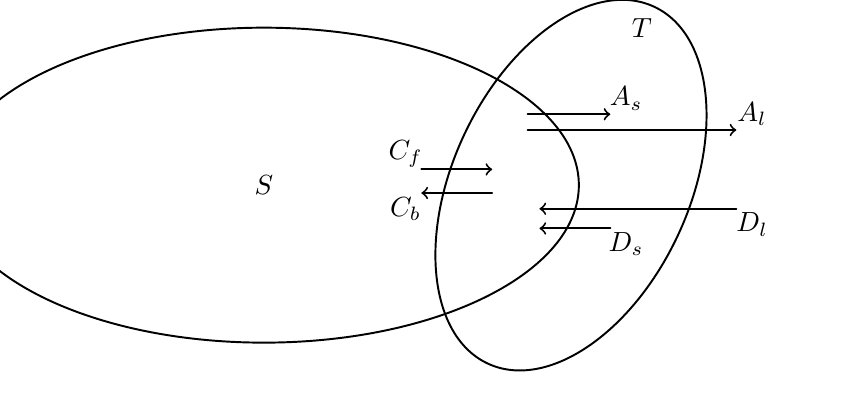
\begin{tikzpicture}[line cap=round,line join=round]
      \path[use as bounding box] (-6, -2.5) rectangle (4, 2);

      \draw[line width=0.7pt] (-3,0) ellipse (4 and 2);
      \draw[] (-3,0) node {$S$};

      \draw[rotate around={65:(0.9,0)}, line width=0.7pt] (0.9,0) ellipse (2.5 and 1.5);
      \draw[] (1.8,2) node {$T$};

      \draw[->, line width=0.7pt] (0.35,0.9) -- (1.4,0.9);
      \draw[] (1.6,1.1) node {$A_s$};

      \draw[->, line width=0.7pt] (0.35,0.7) -- (3,0.7);
      \draw[] (3.2,0.9) node {$A_l$};

      \draw[->, line width=0.7pt] (-0.1,-0.1) -- (-1,-0.1);
      \draw[] (-1.2,-0.3) node {$C_b$};

      \draw[->, line width=0.7pt] (-1,0.2) -- (-0.1,0.2);
      \draw[] (-1.2,0.4) node {$C_f$};

      \draw[->, line width=0.7pt] (1.4,-0.55) -- (0.5,-0.55);
      \draw[] (1.6,-0.75) node {$D_s$};

      \draw[->, line width=0.7pt] (3,-0.3) -- (0.5,-0.3);
      \draw[] (3.2,-0.5) node {$D_l$};

    \end{tikzpicture}
    }
    \end{center}
    \caption{\label{figure:xsp1}
The figure illustrates $S$ and $T$ as used in \hyperref[lemma6-1]{Lemma \ref{lemma6-1}} along with the edges adjacent to $S\cap T$. The names $A_s$ and $A_l$ are meant to read $A$-short and $A$-long, and likewise with $D_s$ and $D_l$.}
  \end{figure}
\end{document}
